%*****************************************************************************************
\part{Identification of Qualitative Sample Properties}
\chapter{Introduction and Motivation}
\ifpdf
    \graphicspath{{Chapter5/Figs/Raster/}{Chapter5/Figs/PDF/}{Chapter5/Figs/}}
\else
    \graphicspath{{Chapter5/Figs/Vector/}{Chapter5/Figs/}}
\fi

%%%%%%%%%%%%%%%%%%%%%%%%%%%%%%%%%%%%%%%%%%%%%%%%%%%%%%%%%%%%%%%%%%%%%%%%%%%%%%%
\section{Introduction}

The second part of the project can be outlined as follows:

\begin{itemize}
    \item Collation of variant locations from Sanger data sets
    \item Construction of script to select a `representative' genomic region
    \item Extraction of regions from whole-genome sequence data
    \item Establishment of leave-one-out analysis pipeline
    \item Comparison of concordance between pipeline results and SNP chip
\end{itemize}

\section{Background}
\subsection{GWAS and iCHIP Data Sets}

As briefly explained in Section~\ref{sec:intro-part2} this part of the project
focuses on measuring the similarity between called variants in pairs of
samples which have been sequenced in different ways. The Sanger Institute has
granted access to a set of human samples which have been sequenced twice, once
with next-generation sequencing (NGS) and the other with SNP genotyping.
The resultant data sets will hereafter be referred to as:

\begin{itemize}
    \item \textbf{GWAS}\footnote{Genome-Wide Association Study} \textit{NGS}\hfill\\
        Every base in the genome of the sample has been sequenced with some
        level of accuracy.
    \item \textbf{iCHIP} \textit{SNP Genotyping}\hfill\\
        Only particular bases of interest in the genome of the sample has been
        sequenced with high accuracy.
\end{itemize}

%TODO Variant Calling
Each sample will thus have a corresponding result from each of the two studies.
A result in this context refers to the output from a variant calling pipeline
at the Sanger Institute -- a \textbf{VCF} file (introduced in
Chapter~\ref{chap:part2:input}) detailing variant sites that were located during
analysis of the sequenced sample.


\subsection{The `Goldilocks' Region}
%TODO Reads a bit poorly

For the next step of the project we are looking to document what effects lanelet
quality has on analysis that occurs downstream from whole-genome sequencing. To
investigate this I'll be performing a leave-one-out analysis on the
\textbf{GWAS} data set: consisting of leaving a particular lanelet out,
re-performing variant calling and comparing the resulting variants called for
each sample to their corresponding \textbf{iCHIP} variants.

The basic idea is to answer the question of what constitutes "good" or
"bad" lanelet quality. Does leaving out a lanelet from the full sequence data
lead to variant calls that better match the SNP chip data, or cause the
correspondence between the two sets to decrease? In which case, having
identified such lanelets, can we look back to the quality parameters we’ve been
analysing so far and find whether they have something in common in those cases?

If we can, these parameters can be used to identify "good" or "bad" lanelets
straight out of the machine. We know that lanelets that exhibit these quality
variables will go on to improve or detriment analysis.

However, variant calling is both computationally and time intensive. Whilst the
Sanger Institute has significant computing resources available, the project time
scale is too small to conduct the analysis on thousands of full sequence samples
and thus we must focus on a smaller region of the human genome.

It is for this reason we are looking for what Sanger described as a
"representative autosomal region". The region must not have too many
variants, or too few: a "Goldilocks genome".


\section{Concepts and Terminology}

In the search for the aforementioned "Goldilocks genome", we define the
following terminology:

\subsection{Group}
%TODO Reads a bit poorly

Rather than considering the location of all variants in our samples as a whole,
we may wish to consider how variants are distributed across the two different
data sets we have, namely the \textbf{GWAS} and \textbf{iCHIP} sets. Thus variants
will be considered as members of a \textbf{group}. The group may be
arbitrarily defined but for the purpose of our own analysis the set in which a
variant appears will be considered as its group.

A particular variant location may appear in more than one group.


\subsection{Length and Stride}
\label{sec:lengthstride}

The \textbf{length} of a region represents the number of bases included in the
region and the \textbf{stride} refers to the number of bases to be used as an
offset between the first base of one region and the beginning of the next.

Sensible choices for these parameters will need to be selected after considering
both time and memory.


\subsection{Density}

The \textbf{density} of a region represents the number of variants located
within that region. \textbf{Density} will be recorded for each \textit{group} of
variants.


\subsection{Candidate Regions}

A \textbf{candidate} is a region of \textit{length} bases whose first base falls
on a \textit{stride}. A \textbf{candidate} region will contain some count
(described as the \textit{density}) of variants for each group. In the context
of this project we consider the number of variant locations that fall within
this region for both the \textbf{GWAS} and \textbf{iCHIP} data sets.

\textbf{Candidates} must meet all (any any additional) criteria to be considered.
For example, regions whose first position falls on a base in such a way that the
chromosome ends before a region of \textit{length} can be constructed will
violate the size criteria.


%%%%%%%%%%%%%%%%%%%%%%%%%%%%%%%%%%%%%%%%%%%%%%%%%%%%%%%%%%%%%%%%%%%%%%%%%%%%%%%
\chapter{Materials and Methods}
\section{Input Data and Format}
\label{chap:part2:input}

\subsection{Variant Call Format}

Variant Call Format (\textbf{VCF}) is a (typically compressed) text file...
...containing records
...developed for the 1000 Genomes Project

\subsection{Variant Query File}
\label{sec:vqf}
%TODO

Named such for the command that creates it, the \textbf{Variant Query File} (or
\textit{Query File}) is an input format for populating the candidate searching
script with variants. The file is formed of line-delimited, tab-seperated
entries where the first field consists of a colon-delimited pair representing a
chromosome and position respectively (\textit{e.g.} 1:5000 is the base at
position 5000 on the first chromosome). Other fields may be provided but are
currently ignored.

The \textbf{Query File} is generated by the \textbf{vcf-query} command
(demonstrated in Listing~\ref{list:vquery}) which is a member of the
\textbf{vcftools} collection -- a tool set designed...  specifically... for
handling \textbf{VCF} files.

...although having found this tool, it turns out that \textbf{bcftools}
implements a more performance efficient \textbf{query} function, thanks to
the performance gains as a result of using \textbf{htslib}...
...the command uses exactly the same syntax, as shown in Listing~\ref{list:bquery}.

Note that information on downloading and installing both tool sets can be found
in Appendix~\ref{app:install}.

\begin{listing}[H]
    \caption[vquery]{: Extracting variant positions from a \textbf{VCF} file
    with \textbf{vcftools}}
    \label{list:vquery}
    \begin{minted}[mathescape,
                %linenos,
                numbersep=5pt,
                gobble=8,
                frame=lines,
                framesep=2mm]{bash}
        vcf-query cd.ichip.vcf.gz -f '%CHROM:%POS\t%REF\t%ALT\n'
    \end{minted}
\end{listing}
http://vcftools.sourceforge.net/perl\_module.html
http://www.biostars.org/p/51076/
http://vcftools.sourceforge.net/htslib.html\#query

\begin{listing}[H]
    \caption[bquery]{: Extracting variant positions from a \textbf{VCF} file
    with \textbf{bcftools}}
    \label{list:bquery}
    \begin{minted}[mathescape,
                %linenos,
                numbersep=5pt,
                gobble=8,
                frame=lines,
                framesep=2mm]{bash}
        bcftools query -f '%CHROM:%POS\t%REF\t%ALT\n' cd-seq.vcf.gz > cd-seq.vcf.gz.q
        # ! A faster alternative to using vcftools exists in bcftools ! #
        # Complains about lack of tabix index but still makes the file...
    \end{minted}
\end{listing}



\subsection{Paths File}
\label{sec:pathsfile}

The \textbf{Paths File} is a trivial and esoteric file type used to handle
grouping of \textbf{Variant Query Files}. The format is simple, using lines
beginning with a '\#' to delimit desired file groups. Entries following that
line (until the next group definition) are considered to be a member of that
group. Entries are line-seperated, tab-delimited and consist of only two fields:
a unique slug that serves only for simple user identification of a file,
followed by the the actual file path (relative or absolute).

It is an error to provide a file entry before the first group definition. An
exception will also be raised if a user defines a group more than once or uses a
duplicate slug due to the ambiguity this introduces.

An example can be found in Appendix~\ref{app:pathsfile}.


\section{Development Environment}

Many of the features of the development environment for Part I are just as
applicable to Part II. Differences and additions to the environment described in
Chapter~\ref{part1:dev} are outlined below.

\subsection{Language}

Once again, Python was the language of choice for many of the reasons previously
discussed in Chapter~\ref{part1:dev:lang}. Additionally, Python is useful for
rapid prototyping, thanks partly to its emphasis on readability; concise
syntax, its dynamic type system and extensive standard library; making it a
suitable choice to author a working script in a short time span.

Although performance was more of a concern, with the use of \textbf{NumPy}
(whose mathematical functions are typically wrappers around C or Fortran
implementations) reasonable efficiency was expected to be obtainable.


\subsection{Testing}

%TODO
Given the more traditional development methodology, testing need not follow a
continuous integration style roadmap. A test suite would need to be written to
ensure the components of the script work as intended, simulating input variants
and ensuring the correct candidate region densities are found.


%%%%%%%%%%%%%%%%%%%%%%%%%%%%%%%%%%%%%%%%%%%%%%%%%%%%%%%%%%%%%%%%%%%%%%%%%%%%%%%
\chapter{Goldilocks}

This chapter introduces \textbf{Goldilocks}; the first programming hurdle for
this part of the project. \textbf{Goldilocks} is a Python script designed
specifically to read in and store locations of user-selected variants on the
human genome and to then find regions of a given size on the genome where
variants are of a desired density.


\section{Design}
\subsection{Purpose}
\label{sec:goldilocks-purpose}

Expanding on the introduction, \textbf{Goldilocks} is responsible for parsing
input files that contain chromosome and base position entries (in the format
described in Section~\ref{sec:vqf}). These files can be grouped to pool the set
of unique variants between each file group to treat them as one search space.

For each group, a list of positions for each chromosome is stored in
memory. Once all variants have been loaded \textbf{Goldilocks} is designed to
iterate over each chromosome\footnote{Strictly speaking we are only handling the
22 \textit{autosomes} and ignoring the remaining 2 sex chromsomes
(\textit{allosomes})} and load all of the variants from the lists in to an array
and essentially count the number of variants present (in each group) between a
given start and end position, determined by the arguments specified by the user
as described in Section~\ref{sec:lengthstride}.

This combination of a start and end position and the counts of variants present
inbetween forms the structure of a \textbf{candidate}. Having performed this
search over all the autosomes, candidates can then be ranked by user-specified
criteria related to the density of the counted variants.


\subsection{Format}

\textbf{Goldilocks} is a modestly sized but elegantly complex Python script
which can also serve as a stand-alone module to be imported in to other
programs. Whilst the use case is certainly more esoteric than \textbf{Frontier},
I made the choice to modularise the functionality, in the hope that if an end
user were to find some function of the script particularly useful they may call
it as part of their own program.


\subsection{Method}
%TODO Add more here?

\textbf{Goldilocks} had to be constructed quickly but carefully. Although
avoiding a quick and dirty solution, the early codebase was arguably cluttered
with blocks of repeated code to perform similar actions for different hard coded
groups. Initial testing was not automated and utilised eyeballing of resulting
data and occasional checking of input files to ensure results were as expected.

Development was akin to a more traditional methodology; requirements were simple
and available up front and formal testing was scheduled to be completed
following the completion of a working prototype.


\subsection{Pitfalls}

Python lists and other sequence based structures such as \textbf{NumPy} arrays
are 0-indexed, however base positions in a genome are commonly 1-indexed. These
differing indices must be normalised in some fashion; for example subtracting 1
from all positions or simply ignoring the presence of element 0 in
the structure. The method that is used does not matter so much as consistency;
it is trivially easy to make 1-base-out mistakes when handling genomic data.

Of note also; after a discussion with the Sanger Institute it has been decided
to exclude candidates located on chromosome 6 from being utilised as a
"Goldilocks region". Chromosome 6 contains a system of genes called the
Human Leukocyte Antigen (HLA)\footnote{A much younger version of me was introduced to
    this concept via the partwork \textit{How Your Body Works}\citep{bodyworks},
    which also distributed English dubs of a 1987 French television show titled
    \textit{Il était une fois... la vie (Once upon a time...
Life)\citep{oncelife}} a relevant episode can be viewed here:
http://www.youtube.com/watch?v=yvhU2UyRv-Q} which encode for Major
Histocompatibility Complex (MHC)\citep{hla-c6}: a critical component of the
body's immune system and of particular importance to anyone requiring an organ
transplant. The HLA can cause difficulties during the variant calling process
due to the high level of variability expressed between samples in these areas
and could thus give less accurate results if we were to measure concordance
using candidates that include these genes.


%%%%%%%%%%%%%%%%%%%%%%%%%%%%%%%%%%%%%%%%%%%%%%%%%%%%%%%%%%%%%%%%%%%%%%%%%%%%%%%
\section{Implementation}

This section considers the implementation of the major components of
\textbf{Goldilocks}:

\begin{itemize}
    \item Handling user defined Paths File
    \item Loading variants from specified Variant Query Files
    \item Storage and recall of variant groups in memory
    \item Searching for candidates with user specified length and stride
    \item Ranking suitable candidates based on variant density
\end{itemize}

\subsection{Input Sanity...?}
%TODO Where to put this? Have another pre-impl section?
Having recovered from the miscommunication that led me to attempt to find
reverse strands in VCF files with already known errors, I’ve been making
performance improvements to the script that finds candidate genomic regions.
The task poses an interesting problem in terms of complexity and memory, as the
human genome is over three billion bases long in total which can easily lead to
data handling impracticalities.


\subsection{Parsing Paths File}
\label{sec:parse-path}

\textbf{Goldilocks} requires the user provide their own valid \textbf{Paths
File}, meeting the specification introduced in Section~\ref{sec:pathsfile} (an
actual example of such a file can be found in Appendix~\ref{app:pathsfile}).

As previously described the file merely documents the locations of the
\textbf{Variant Query Files} to be loaded, along with the desired grouping of
those files. Any variant location that appears in at least one file of a group
will be added to the pooled set of variants for that group.

\textbf{Goldilocks} provides the simple \textbf{load\_variant\_files} to parse
the user's \textbf{Paths File}, where for each group, the following structures are
initialized and added to a dictionaries encapsulated by \textbf{Goldilocks}
itself, using the group name as a key:

\begin{itemize}
    \item \textbf{groups} \textit{Dictionary}\hfill\\
        Keys refer to a particular allosome number, mapped to a list structure
        which will later be populated with the positions of all variants that
        appear on that chromosome in at least one \textbf{Query File} of
        the group. It is from this structure that chromosome \textbf{NumPy}
        arrays will be loaded with data.
    \item \textbf{group\_buckets} \textit{Dictionary}\hfill\\
        Keys refer to a specific number of variants counted (considering only
        variants from the group), mapped to a list
        of all i'th candidate regions which contained that density.
        This structure eases locating groups which match desired density
        criteria once summary statistics have been calculated.
    \item \textbf{group\_counts} \textit{List}\hfill\\
        The number of variants which appear in each candidate, for this variant
        group will be appended to this list.  This structure simplifies the
        gathering of summary data (such as mean, median and variance) of all the
        candidate regions of the group once the search has completed.
\end{itemize}

A \textbf{Paths File} which violates the specification will raise an exception
during execution of this function, informing the end user of their error. This
was decided to ensure ambiguous input did not cause confusion later, for example
should defining a file group twice merge or override the first
definition?


\subsection{Loading Variant Query Files}
%TODO Figure:
%
%     groups [ ][ ][ ][ ][ ]...
%     group  [ ]
%     chrom   \
%              [][][][][][]...
%              |
%     indexes  [0,1,2,3...]
%

\textbf{load\_variants\_from\_file} is responsible for loading a given
\textbf{Variant Query File} and adding the position of each record contained
within to the appropriate group-chromosome list pair in the \textbf{groups}
structure.

It is important to note that this function is not responsible for
ensuring the positions added to the list are unique to avoid performance
penalties in checking whether a variant is already a member of the list (which
increase proportionally for the size of the list).
However as examined in Section~\ref{sec:python-structures}, appending a
significant number of items to a list will likely induce costly memory
operations as the list is resized. Thus use of a set might have been more
appropriate (especially considering the container forbids duplicate entries)
but a set must be constructed from an existing iterable such as a list anyway!

Indeed the container does specify an \textbf{update} function but this could in
itself be a source of overhead as the structure ensures that the no duplicate
condition has not been violated on every call. Given more time it would be
interesting to compare performance differences between container implementations.

%TODO Sound ok?
\textbf{load\_variants\_from\_file} has another responsibility in keeping track
of the "furthest along" variant position for each chromosome across all groups,
this is used in the search step later, firstly to ensure that candidates are not
constructed beyond where the last variant on a chromosome lies (as by definition
they would be empty and searching over them would waste resources) and secondly
to normalize the candidate regions across all groups to allow for easy
comparison between them.


\subsection{Storage and Recall of Variants}

As I discussed previously, on the hunt for my Goldilocks genomic region, it is
important to consider both time and memory as it is simple to deliver a poor
performing solution.

Searching for candidates regions over the entire genome at once is probably
unwise. Luckily, since our candidate must not span chromosomes (telomeres --
the ends of chromosomes are not very good for reads) then we can easily yield a
great improvement from processing chromosomes individually.

The process is to extract the locations of all the variants across the genome
from the SNP chip VCF files (these files list the alleles for each detected
variant for each sample), load them in to some sort of structure, “stride” over
each chromosome (with some stride offset) and finally list the variants present
between the stride start and stride start plus the desired length of the
candidate. These are our regions.

Due to the use of striding, one does not simply walk the chromosome. A quick
and dirty solution would be to just look up variants in a list:

\begin{minted}[mathescape,
            %linenos,
            numbersep=5pt,
            gobble=4,
            frame=lines,
            framesep=2mm]{python}
    for chromosome in autosomes:
        for start in range(1, len(chromosome), STRIDE):
            for position in range(start, start+LENGTH):
                if position in variant_position_list:
                    # Do something...
\end{minted}

This is of course rather dumb. Looking up a list has $\mathcal{O}$(n) performance
where n is the number of variants (and there are a lot of variants). Combining
this with the sheer number of lookups performed, with the default parameters the
list would be queried half a billion times for the first chromosome alone.

You could improve this somewhat by dividing the variant\_position\_list in to a
list of variants for each chromosome, so at least n is smaller. It is pretty
doubtful that this would make any useful impact given the number of lookups.
I’m happy to say I bypassed this option but thought it would be fun to consider
its performance.

A far more sensible solution is to replace the list with a dictionary
whose lookup is amortized to a constant time. The number of lookups is still
incredibly substantial but a constant lookup is starting to make this sound
viable. Using the variant positions as keys of a dictionary (in fact let us use
the previous minor suggestion and have a dictionary for each chromosome) we
have:

\begin{minted}[mathescape,
            %linenos,
            numbersep=5pt,
            gobble=4,
            frame=lines,
            framesep=2mm]{python}
    for chromosome in autosomes:
        for start in range(1, len(chromosome), STRIDE):
            for position in range(start, start+LENGTH):
                if position in variant_position_dict[chromosome]:
                    # Do something...
\end{minted}

This still takes half an hour to run on my laptop though, surely there
is a better way.  I wondered if whether dropping the lookup would improve
things. Instead, how about an area of memory is allocated to house the current
chromosome and act as a variant “mask” -- essentially an array where each element
is a base of the current chromosome and the value of 1 represents a variant at
that position and a 0 represents no variant.

\begin{minted}[mathescape,
            %linenos,
            numbersep=5pt,
            gobble=4,
            frame=lines,
            framesep=2mm]{python}
    for chromosome in autosomes:
        chro = np.zeros(len(chromosome), np.int8)
        for variant_loc in snps_by_chromosome[chromosome]:
            chro[variant_loc] = 1

        for start in range(1, len(chromosome), STRIDE):
            for position in range(start, start+LENGTH):
                if chro[position] == 1:
                    # Do something...
\end{minted}

We of course have to initially load the variants in to the chromosome array,
but this need only be done once (per chromosome) and is nothing compared to the
billions of lookups of the previous implementation.

Rather to my surprise this was slow  (maybe if I have time I should
check how it compared to looking up with a list). Was it the allocation of
memory? Perhaps I had run out of RAM and most of the work was going in to
fetching and storing data in swap?

I switched out the comparison (== 1) step for the previous dictionary based
lookup and the performance improved considerably. What was going on? There must
be more to looking at a given element in the numpy chromosome array, but what?

After a brief spell of playing with Python profilers and crashing my laptop by
allocating considerably more memory than I had with numpy.zeroes, I read the
manual (!) and discovered that numpy.zeroes returns an ndarray which uses
“advanced indexing” even for single element access, effectively copying the
element to a Python scalar for comparison.

That’s a lot of memory action.

It then occurred to me that we’re interested in just how many variants are
inside each region and our chromosome is handily encapsulated in a numpy array.
Why don’t we just sum together the elements in each region? Remember variant
positive base positions are 1 and 0 otherwise, useful. So the work boils down
to some clever vector mathematics calculated by numpy.

We don’t even lose any detail because the actual list of variants inside a
region can be recovered in a small amount of time just given the start and end
position of the region.

\begin{minted}[mathescape,
            %linenos,
            numbersep=5pt,
            gobble=4,
            frame=lines,
            framesep=2mm]{python}
    for chromosome in autosomes:
        chro = np.zeros(len(chromosome), np.int8)
        for variant_loc in snps_by_chromosome[chromosome]:
            chro[variant_loc] = 1

        for start in range(1, len(chromosome), STRIDE):
            num_variants = np.sum(chro[start:start+LENGTH])
            # Do something...
\end{minted}

With conservative testing this runs at least 60 times faster than before, the
entirety of the human genome can be analysed for candidate regions in less than
twenty seconds (with the first few seconds taken reading in all the variant
locations in the first place).

...Ignoring empty regions etc.

\begin{minted}[mathescape,
            %linenos,
            numbersep=5pt,
            gobble=4,
            frame=lines,
            framesep=2mm]{python}
    def load_chromosome(self, size, locations):
        chro = np.zeros(size+1, np.int8)

        # Populate the chromosome array with 1 for each position a variant exists
        for variant_loc in locations:
            chro[variant_loc] = 1

        return chro
\end{minted}

\textbf{load\_chromosome} returns a \textbf{numpy} array representing the
chromosome, given its desired length and a list of variants...

%FUTURE
...supervisor suggested bloom filters...
...would be a useful experiment to measure what further performance gains could
be acheived with such a method...


\subsection{Searching for Candidate Regions}

\textbf{search\_regions} is responsible for performing the main task of the
script, walking over the genome and creating objects who represent candidate
regions. The function is possibly a misnomer as it conducts a candidate census
rather than a search, indiscriminately adding all valid candidates to the
\textbf{regions} dictionary.

\textbf{search\_regions} will iterate over each chromosome and load the listed
variants in each group-chromosome pair from the \textbf{groups} structure (by
calling \textbf{load\_chromosome}) into a
\textbf{NumPy} array whose length is set to the last position from which a full
region can be extracted based on the maximum position seen by
\textbf{load\_variants\_from\_file} for this chromosome, plus one to account for
the 1-indexed nature of genome positions. The function will then take slices of
these arrays of the user defined \textit{length} and count the number of
variants contained within by summing across the slice (elements with variants
contain a 1, otherwise 0). The next region is sliced by moving the first base of
the current region forward by the user defined \textit{stride}.

Each valid region will be entered in to the \textbf{regions} dictionary using
the current region counter (\textbf{region\_i}) as the key, mapping to an
arbitrary object (a dictionary) as defined in Listing~\ref{list:candidate-dict}
below:

\begin{listing}[H]
    \caption[candidate-dict]{: Candidate Region Data Structure}
    \label{list:candidate-dict}
    \begin{minted}[%mathescape,
                %linenos,
                gobble=8,
                frame=lines,
                framesep=2mm]{python}
        regions[region_i] = {
            "ichr": i,              # The i'th region on the current chromosome
            "group_counts": {},     # A dictionary mapping variant group names to
                                    # the number of variants counted for that group
            "chr": chrno,           # The allosome number
            "pos_start": region_s,  # The first base of this region (inclusive)
            "pos_end": region_e     # The last base on this region (inclusive)
        }
    \end{minted}
\end{listing}

Regions will also have their respective group densities appended to the
appropriate \textbf{group\_counts} list and its \textbf{region\_i} added to the
relevant \textbf{group\_buckets} structure as established in
Section~\ref{sec:parse-path}.


\subsection{Filtering and Ranking Candidates for Selection}
\label{sec:filter-rank}

For the purpose of this project we're looking to filter candidates by their
absolute distance from the median density of variants located in the
\textbf{GWAS} variant group (the median density will give the most representative
regions) and then rank those by their corresponding \textbf{iCHIP} variant group
densities, descending (enriching the number of comparisons that can be made
between the \textbf{GWAS} data and \textbf{iCHIP} data).

Two functions in the \textbf{Goldilocks} API provide a process to rank candidate
regions by a desired group's density:

\begin{itemize}
    \item \textbf{initial\_filter} \hfill\\
        Uses the relevant filtering group's \textbf{group\_counts} list (in this case,
        \textbf{GWAS}) to calculate a window around the median density. The
        function will then return all candidates inside the group's
        \textbf{group\_buckets} dictionary whose density fall inside the upper
        and lower bounds of the window around the median.

    \item \textbf{enrich} \hfill\\
        Sorts the output of \textbf{initial\_filter} by the desired ranking
        variant group (in our case, \textbf{iCHIP}). The function will
        prioritise candidates with the closest absolute value to the filter group's median
        and ensure that the density of the ranking group is higher than the
        filtering group. Returns a ranked list of candidates in the format
        displayed in Listing~\ref{list:candidate-dict} for manual inspection.
\end{itemize}

Currently ranking and filtering criteria are still hard coded to meet the needs
of our analysis.  In future it would be useful to generalise the
\textbf{Goldilocks} API to allow more operations such as filtering by a given
percentile rather than only the median and to provide more 'enrichment' options
such as ranking by minimum.

It would be sensible to consider re-naming the two functions to \textbf{filter}
and \textbf{rank} respectively and allow users to chain together these methods
to compound filtering and ranking operations as necessary.

Whilst in this state the script proposes little re-use value, we at least have a
basis for repeating results in future with different data sets or additional
variant groups.


%%%%%%%%%%%%%%%%%%%%%%%%%%%%%%%%%%%%%%%%%%%%%%%%%%%%%%%%%%%%%%%%%%%%%%%%%%%%%%%

\section{Testing}

The testing of \textbf{Goldilocks} presented a challenge; we'd not only like
to simply ensure that the correct query files are located and loaded in to
memory but also that the expected candidates are found, filtered and selected.
It is thus not practical to conduct testing on a large data set such as the two
we have for analysis, we need a smaller, well defined set with known results.

To acheive this the testing suite is designed to generate valid
\textbf{Variant Query Files} from a \textbf{TEST\_DATA} dictionary, which
defines test groups and variant locations on test chromosomes and can easily be
altered for future testing. Test files are re-generated from this dictionary
each time the test suite is instantiated using the \textbf{setUpClass}
classmethod provided by the \textbf{unittest} library.

Checking both the \textbf{Paths File} and generated \textbf{Variant Query Files}
were loaded successfully is trivial and the suite goes on to test whether the
input files and all generated variants within are mapped to the specified
chromosome of the correct group, both in memory and also when loaded in to the
\textbf{NumPy} array structure. Once regions have been searched (or more
accurately, once a a candidate census has populated the \textbf{regions}
dictionary via \textbf{search\_regions}), additional tests ensure that all
candidate regions are of the correct \textit{length} and begin on a valid
\textit{stride}.

%TODO Center
\begin{listing}[H]
    \caption[test-gold]{\textbf{Testing Expected Candidates with Goldilocks}:
    The test suite defines the locations of variants across many files in two
groups, the figure represents the expected regions for \textit{GROUP0}. The
horizontal line represents a particular chromosome on which a \textbf{*} signals
the location of a variant (\textbf{=} otherwise). The expected size column
tabulates the number of variants that should appear as a member of region i
(start-end inclusive).}
    \label{list:test-gold}
    \begin{minted}[%mathescape,
                %linenos,
                fontsize=\scriptsize,
                gobble=0,
                frame=lines,
                framesep=2mm]{text}
 GROUP0
 CHR 1                                                            Expected
             4     10 13      21  25                                Size    i
       1 |*==*=====*==*=======*===*========================*| 50
          |        |                                                 3      0
               |        |                                            2      1
                    |        |                                       1      2
                         |        |                                  2      3
                              |        |                             2      4
                                   |        |                        0      5
                                        |        |                   0      6
                                             |        |              0      7
                                                  |        |         1      8
                                                       |        |    x

 GROUP0
 CHR 2                                                            Expected
              5                                   91                Size    i
       1 |====*=================\/...\/===========**********| 100
          |        |                                                 1      9
               |        |                                            0      10
                                  ...                                .      .
                                             |        |              5      26
                                                  |        |         10     27
                                                       |        |    x

    \end{minted}
\end{listing}

As discussed, testing the discovery of correct regions is more complex.
Listing~\ref{list:test-gold} details the regions expected for the variants
specified in \textbf{TEST\_DATA}. The test suite checks that the number of
regions located and their content is correct for each chromosome in each variant
group. Tests also ensure that the previously mentioned \textbf{group\_counts}
and \textbf{group\_buckets} structures are populated appropriately.

Finally the \textbf{initial\_filter} and \textbf{enrich} functions can be tested
(as we are able to manually calculate the expected candidates given the small
data set) and ensure those candidates are returned.

Admittedly the suite could still be described as modest and with more time it
would be appropriate to further improve coverage, possibly generating larger (or
even random) data sets. Results however, have also undergone manual inspection
both by myself and the Sanger Institute and the regions described in
the following chapter are considered legitimate.


%%%%%%%%%%%%%%%%%%%%%%%%%%%%%%%%%%%%%%%%%%%%%%%%%%%%%%%%%%%%%%%%%%%%%%%%%%%%%%%
\chapter{Results}
%TODO Mnt or Mb?
%TODO Tabulate

Listing~\ref{list:resultsp2} lists the top 25 candidate regions selected by
\textbf{Goldilocks} for inspection. Regions were constructed using a
\textit{length} of 1Mnt\footnote{1,000,000 bases}(mega nucleotides) and a
\textit{stride} of 0.5Mnt\footnote{500,000 bases}. As detailed in
Section~\ref{sec:filter-rank}, candidates for this study were filtered to
include regions with a \textbf{GWAS} density within ±12.5\% of the
median \textbf{GWAS} density (\textit{i.e.} in the middle 25\%) before being
ranked firstly by absolute difference from the median \textbf{GWAS}, then by
\textbf{iCHIP} variant density, descending.

Empty regions were excluded from a variant group's analysis, including the
calculation of any percentiles. This was to ensure that we located the most
"representative" density from the regions and avoid potential skewing from 0 density
candidates. However repeating the experiment including empty regions
leads to highly similar results and the candidate that was actually selected as
the Goldilocks region appears in both sets of results.

%TODO Results don't actually sub-sort by iCHIP...
\begin{listing}[H]
    \caption[resultsp2]{\textbf{Goldilocks Results}: "Top 25" Candidate Regions
    using a \textit{length} of 1Mnt and a \textit{stride} of 0.5Mnt. Candidates
    are filtered by median \textbf{GWAS} density and ranked by maximum
    \textbf{iCHIP} density.}
    \label{list:resultsp2}
    \begin{minted}[%mathescape,
                %linenos,
                gobble=8,
                frame=lines,
                fontsize=\scriptsize,
                framesep=2mm]{text}
        i	GWAS	iCHIP	CHR	POSITIONS
        0234	297	470	1	 117000001 -  118000000
        1074*	294	1540	3	  46000001 -   47000000
        5222	294	336	21	  16500001 -   17500000
        3125	298	310	10	  60000001 -   61000000
        0880	293	344	2	 191500001 -  192500000
        3560	299	772	12	   9000001 -   10000000
        4407	299	512	15	  78500001 -   79500000
        1036	292	300	3	  27000001 -   28000000
        2734	300	515	9	   5000001 -    6000000
        3426	300	486	11	  76000001 -   77000000
        0015	291	1029	1	   7500001 -    8500000
        0365	301	487	1	 182500001 -  183500000
        3415	301	419	11	  70500001 -   71500000
        1581	290	802	4	 102500001 -  103500000
        3554	290	403	12	   6000001 -    7000000
        3184	302	449	10	  89500001 -   90500000
        1580	289	603	4	 102000001 -  103000000
        1948	288	1297	5	  96000001 -   97000000
        2215	288	622	7	  49500001 -   50500000
        0414	288	346	1	 207000001 -  208000000
        2055	304	1377	5	 149500001 -  150500000
        0384	287	827	1	 192000001 -  193000000
        0959	306	406	2	 231000001 -  232000000
        4214	286	393	14	  88500001 -   89500000
        0320	307	620	1	 160000001 -  161000000
    \end{minted}
\end{listing}

%TODO Possible all returned variants?
Candidate 1074 (marked by \textbf{*}) was selected as the region with the
closest absolute difference between the median \textbf{GWAS} density of 297,
whilst also offering the highest \textbf{iCHIP} density of the top 25 returned
candidates.


The implementation of the filtering and ranking functions in the previous
chapter noted that during final ranking, the \textbf{enrich} function will
discard candidates if the number of variants in the ranking group is less than
the filtering group -- in this case, if the \textbf{iCHIP} density is lower than
the \textbf{GWAS}. This was a crude rule implemented to prevent candidates with
a significantly low \textbf{iCHIP} density ($\le$100) from being put forward following
'enrichment'; these regions would give us little to compare when it comes to
measuring the concordance between variants called in our leave-one-out study and
the original \textbf{iCHIP} data set.

Curious about the wide range and presence of so many low resolution
\textbf{iCHIP} candidates, I authored an R script (making use of
\textbf{ggplot2}\citep{ggplot2} for graphing) to plot
figures~\ref{fig:megabaseplot} and~\ref{fig:megabaseplotsplit} as a means of
visual inspection to confirm such results should be anticipated.

Figure~\ref{fig:megabaseplot} shows a large range in the densities of
variants in the \textbf{iCHIP} regions, between 0 and almost 3000, with a
significant baseline below 100. Figure~\ref{fig:megabaseplotsplit} plots the
same data set but also facetting by chromosome, again it can be seen that the
\textbf{iCHIP} variant group counts are well spread when compared to the rather
constant variance of their \textbf{GWAS} counterparts.

This isn't a surprise when you consider that the \textbf{GWAS} data set
represents the variants sequenced from whole-genome analysis of our samples,
whereas the \textbf{iCHIP} set consists of the variants output from SNP
genotyping, a process that focuses on particular genomic locations of interest.


\begin{figure}[htbp!]
    \centering
    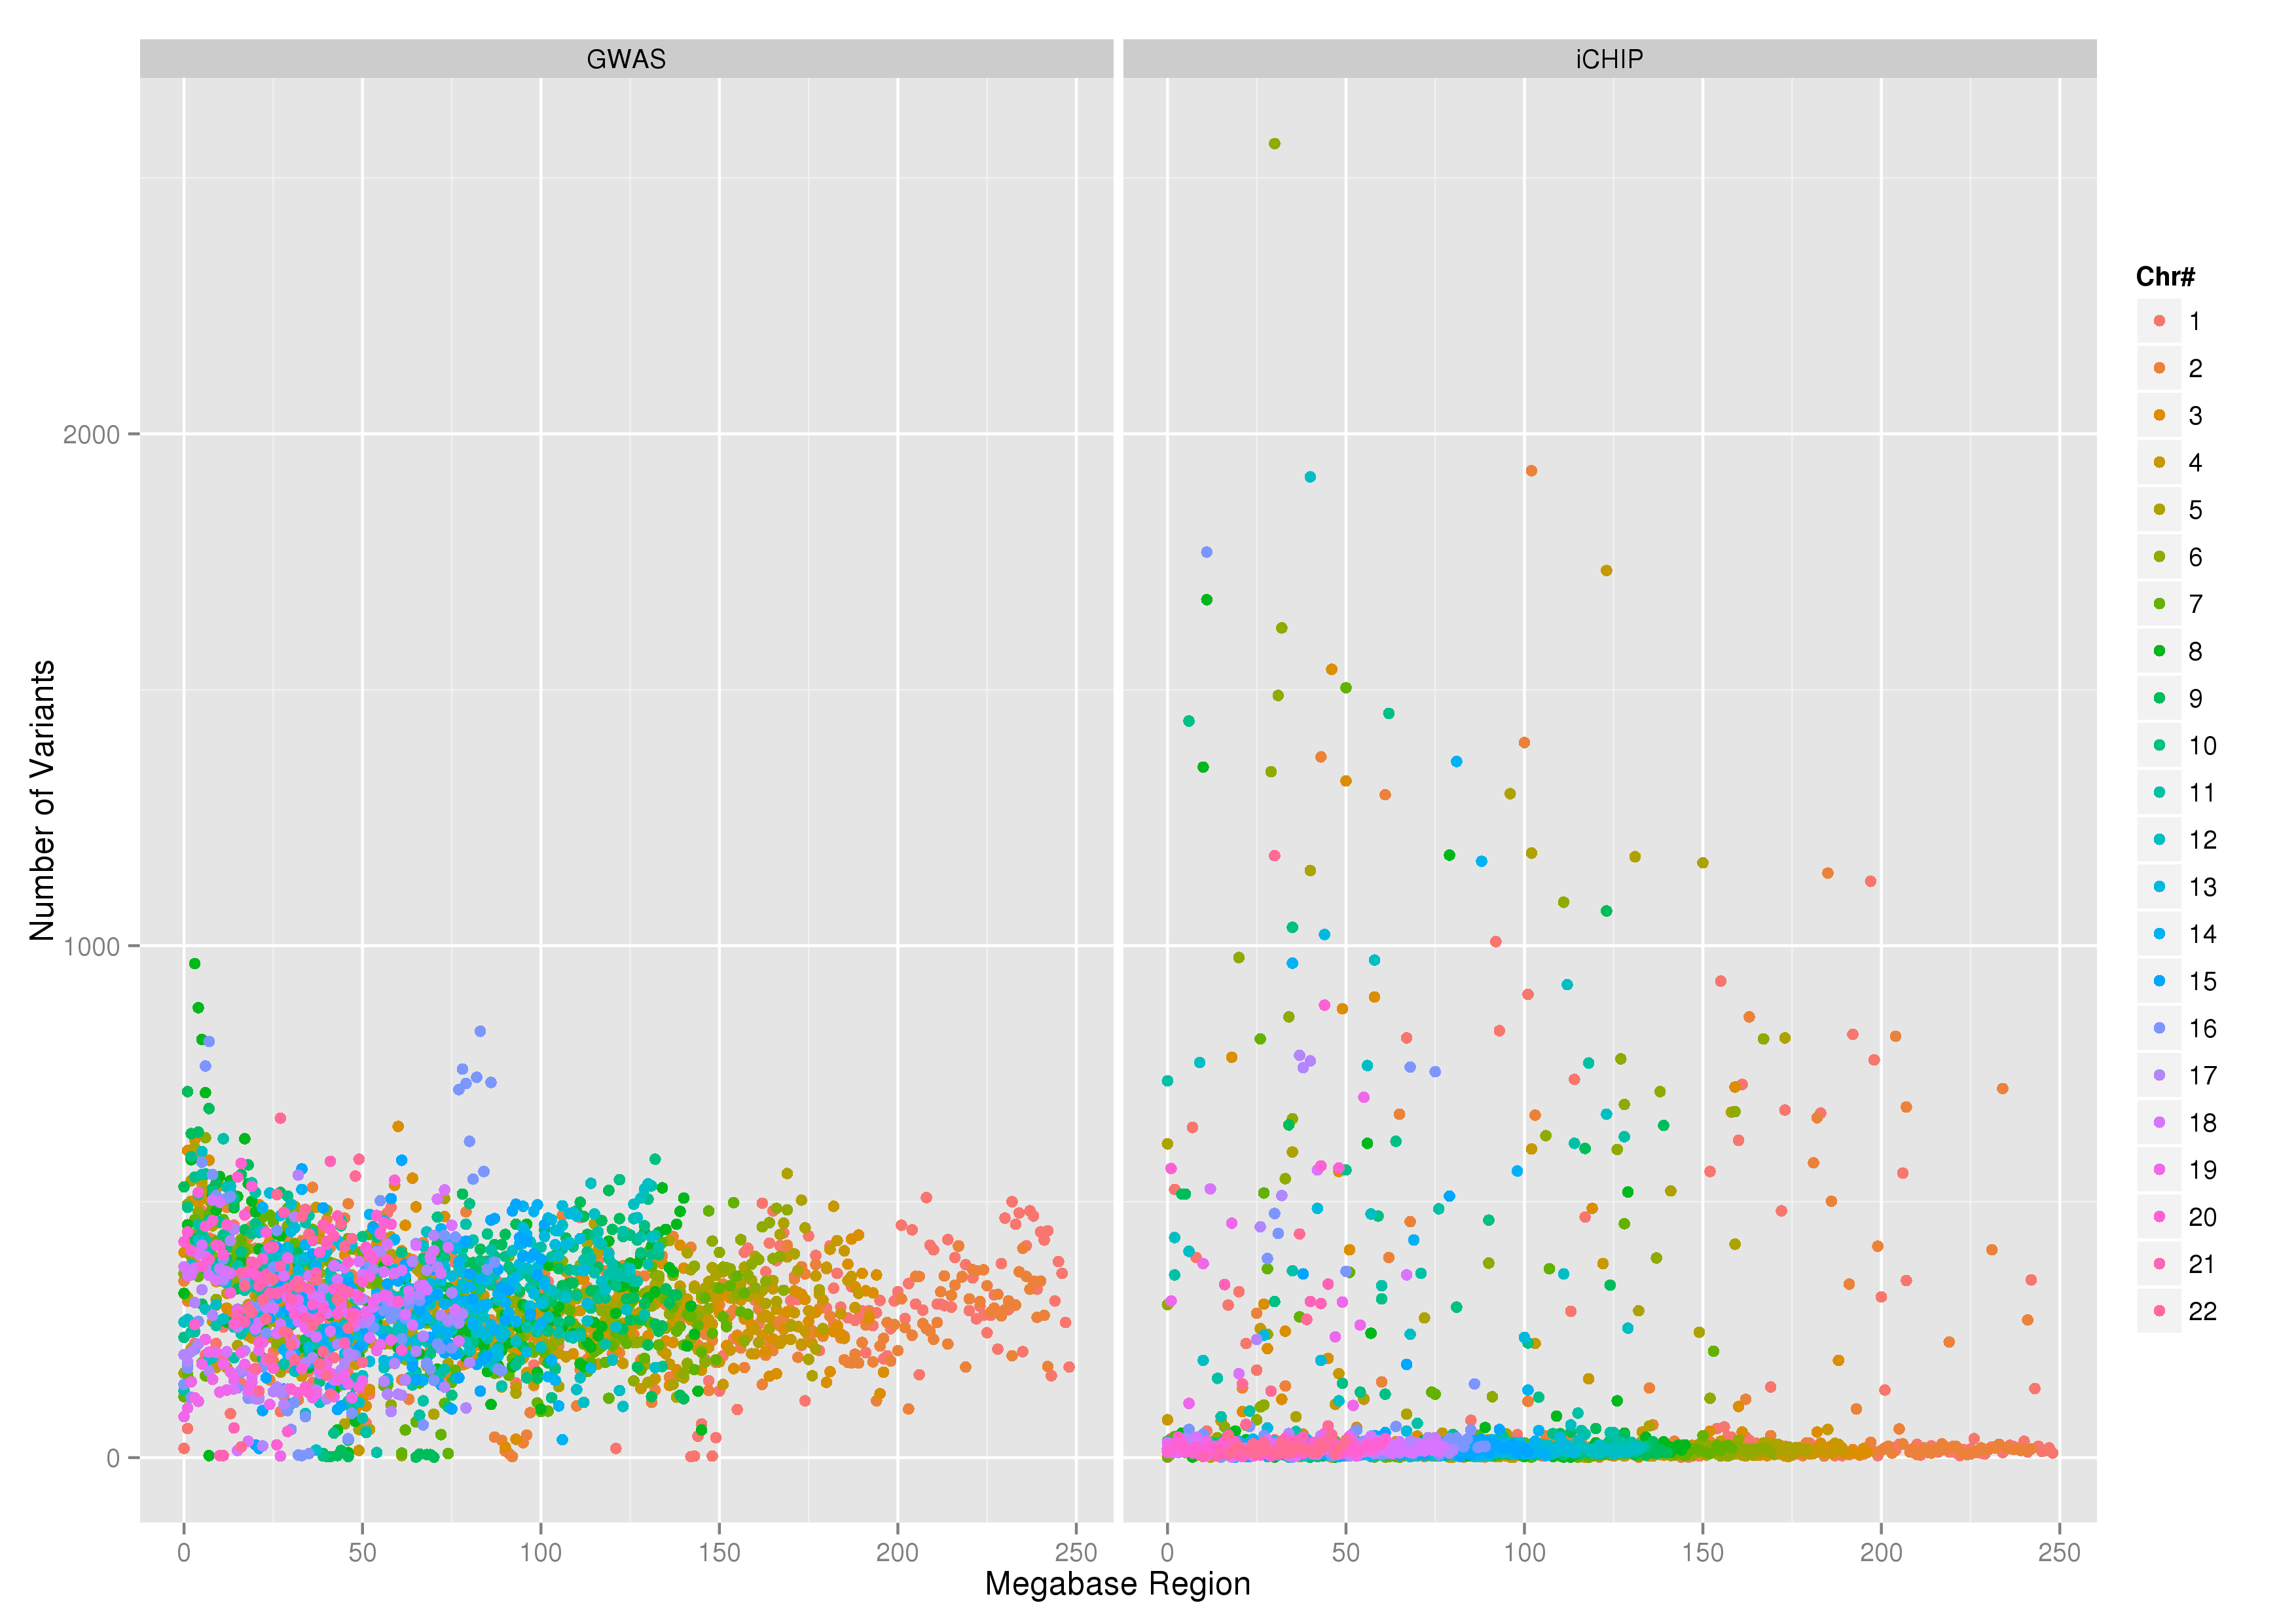
\includegraphics[width=0.8\textwidth]{megabase_plot}
    \caption[megabaseplot]{\textbf{Goldilocks Candidate Plot A}: Candidate regions
    of one megabase length are arranged along the x axis (coloured by
chromosome) against the number of variants contained within that region.}
    \label{fig:megabaseplot}
\end{figure}
\begin{figure}[htbp!]
    \centering
    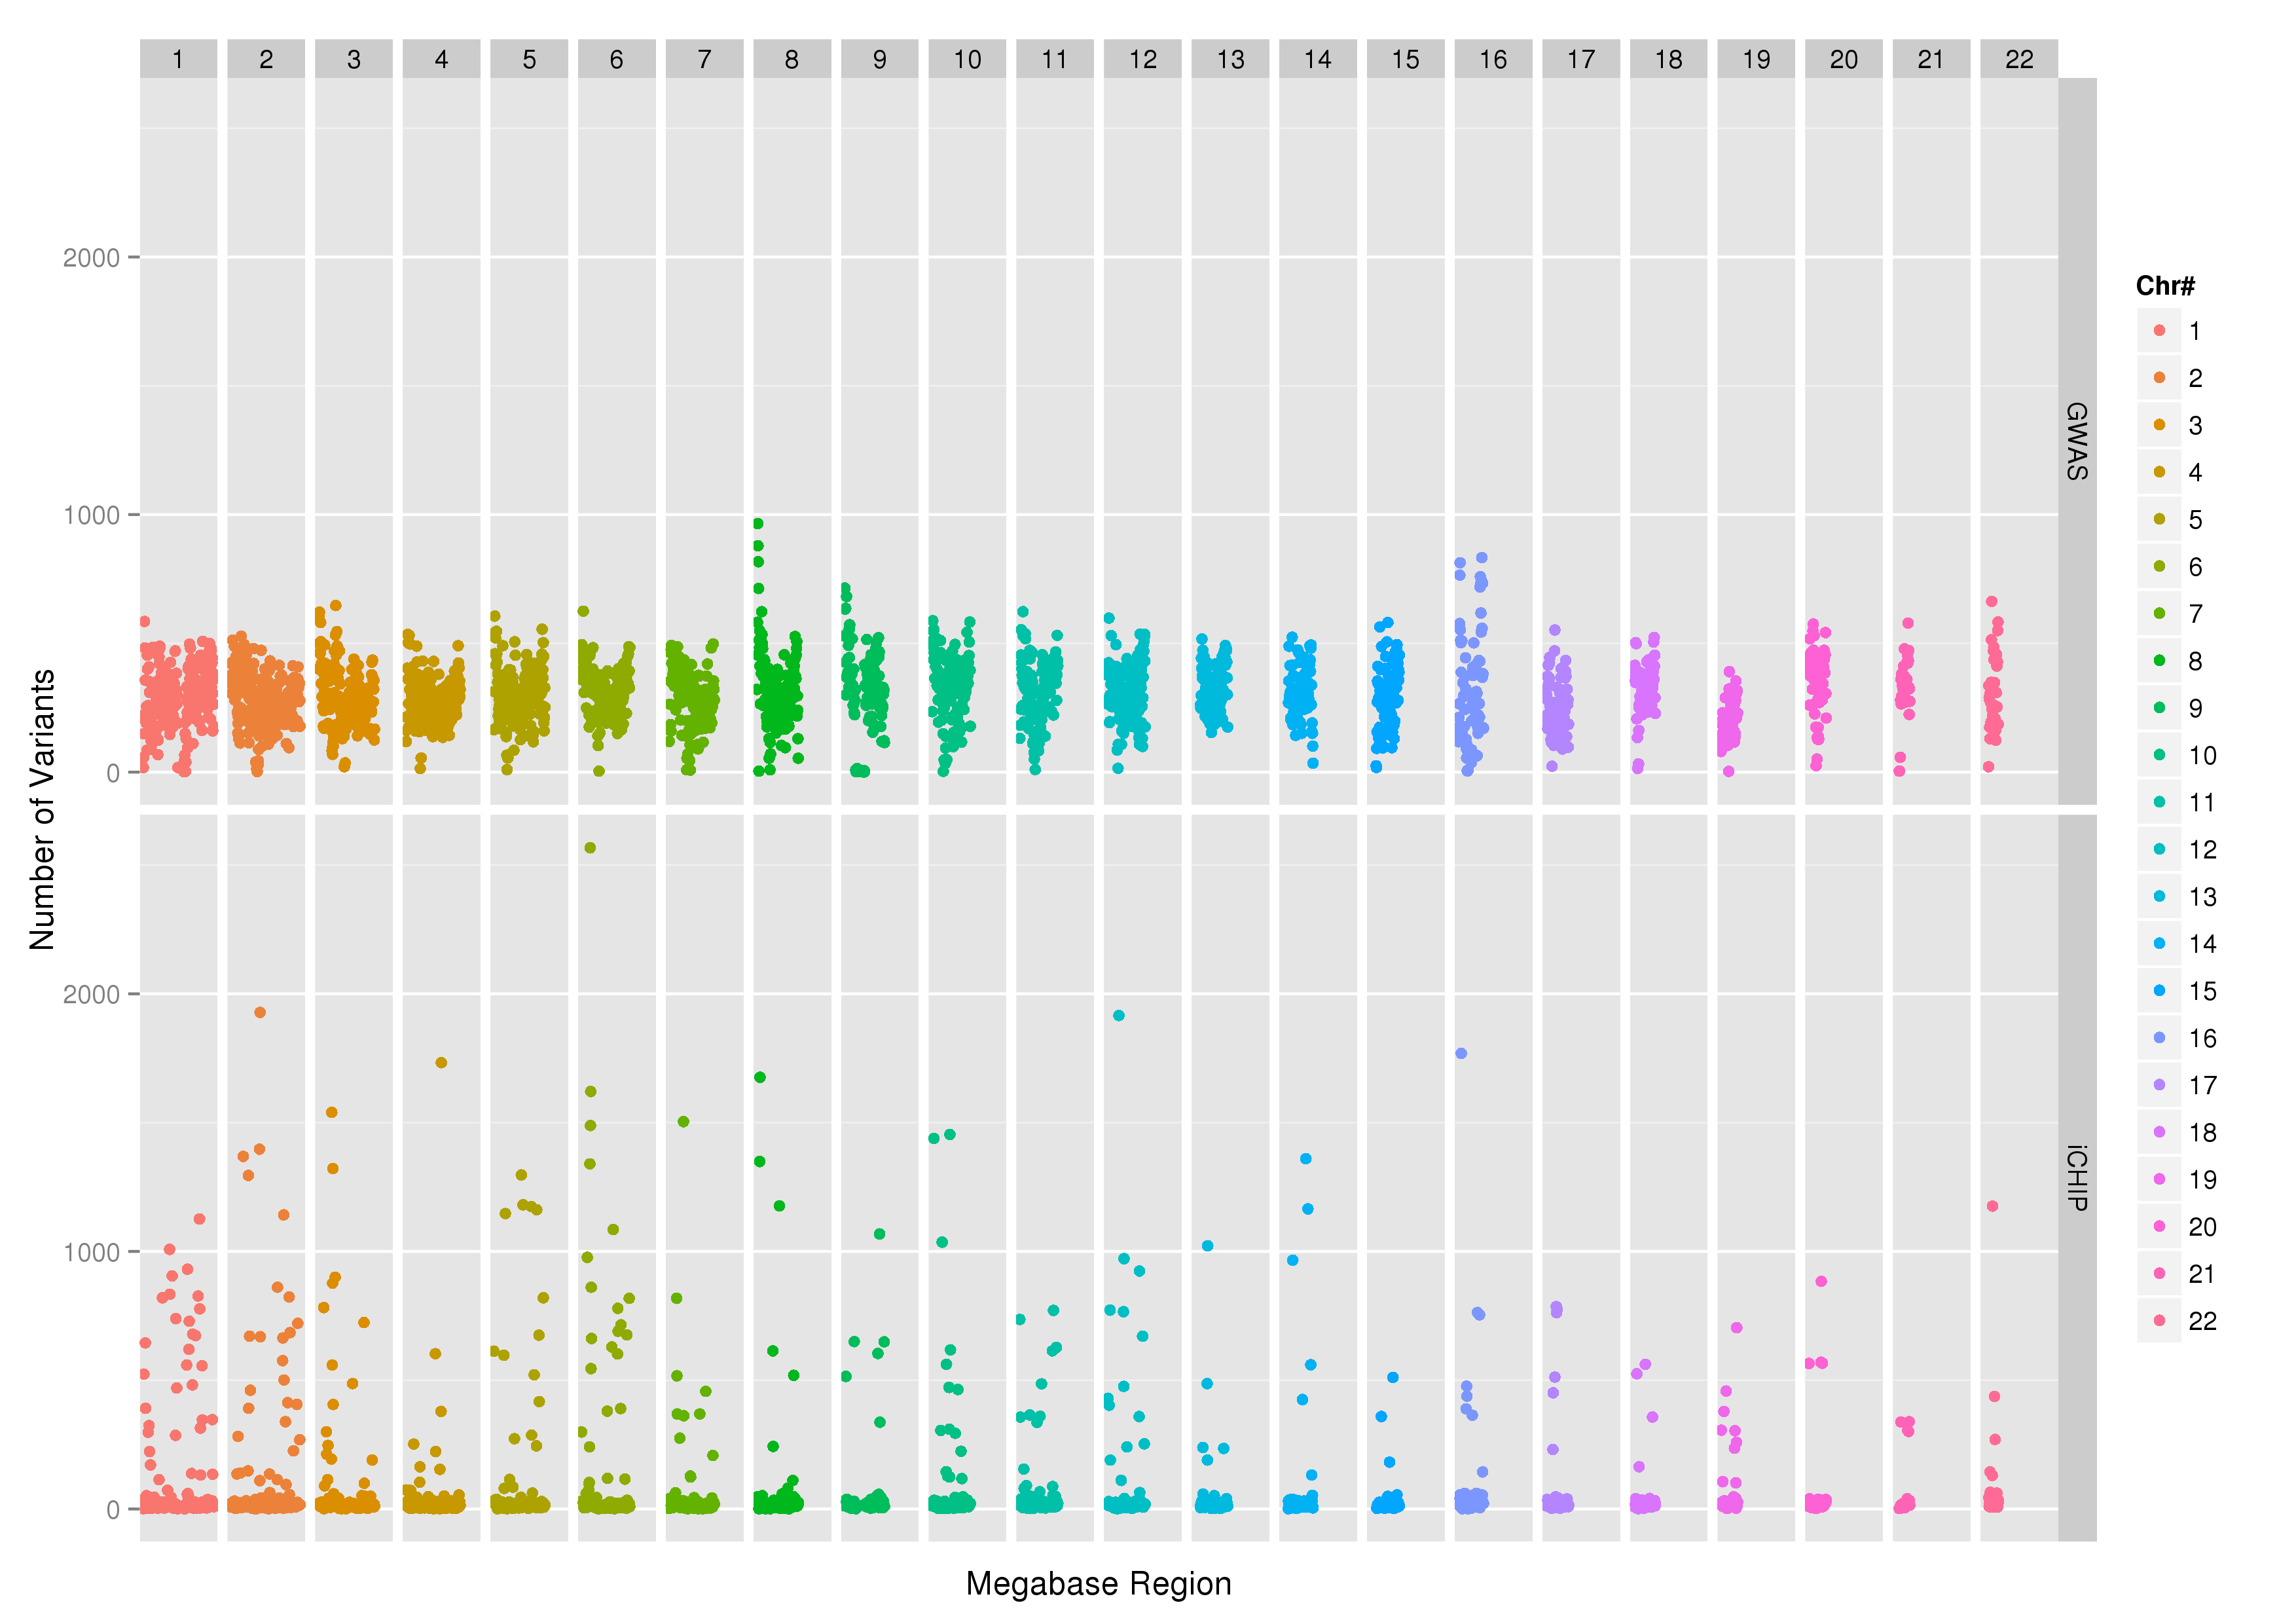
\includegraphics[width=0.8\textwidth]{megabase_plot_split}
    \caption[megabaseplotsplit]{\textbf{Goldilocks Candidate Plot B}: Candidates
        of one megabase length are arranged along the x axis (coloured
        and facetted by allosome) and plotted against the number of variants contained
    within that region.}
    \label{fig:megabaseplotsplit}
\end{figure}


%%%%%%%%%%%%%%%%%%%%%%%%%%%%%%%%%%%%%%%%%%%%%%%%%%%%%%%%%%%%%%%%%%%%%%%%%%%%%%%
\chapter{Analysis Pipeline}
%TODO Have we explained pipeline yet?

Having selected the Goldilocks region (Chromosome 3: 46,000,001---47,000,000)
via \textbf{Goldilocks}, we must now begin constructing the pipeline that will
conduct the leave-one-out analysis over all the \textbf{GWAS} lanelets and
compare the called variants to the appropriate \textbf{iCHIP} sample.

This chapter introduces the various components of the pipeline, their purpose
and any difficulties encountered.

\section{Overview}

%TODO Design section?
%TODO Flow chart!

The pipeline can be divided up in to the following analysis steps:

%TODO Are we taking these from the lanelets?
%TODO What file formats?
% http://biobits.org/samtools_primer.html
% TODO Improve descriptions here...
\begin{itemize}
    \item \textbf{Extraction} \hfill\\
        For every whole-genome lanelet from the \textbf{GWAS} study, extract the
        Goldilocks region.
    \item \textbf{Indexing} \hfill\\
        %TODO Cite performance improvements, better explanation
        Create indexes for the extracted Goldilocks regions, improving
        efficiency for tools which require random access to variants inside the
        region.
    \item \textbf{Merge} \hfill\\
        Merge the data from each extracted region in to one file to reduce file
        handling overhead in later analysis.
    \item \textbf{Pileup} \hfill\\
        %TODO Mention probabilities...
        Calculate genotype likelihoods based on the reads seen across all the
        extracted Goldilocks regions.
    \item \textbf{Call} \hfill\\
        Use the genotype likelihood scores to actually call the variants for
        each position of interest in each of the Goldilocks regions.
    \item \textbf{Compare} \hfill\\
        %TODO Lanelets, samples, what are we doing?
        % Are lanelets combined in to one sample for comparison?
        For each pair of \textbf{GWAS} and \textbf{iCHIP} samples, measure the
        concordance of called variants.
\end{itemize}

%The first two steps need only be conducted once.
\section{Concepts and Terminology}
%TODO Concepts: Genotype Likelihood?

\subsection{htslib}
...high-throughput sequencing library...

\subsection{samtools}
\subsection{bcftools}
...spun off from the \textbf{samtools} repository...
...now using \textbf{htslib}...

\subsection{SAM and BAM Files}

\subsection{"The Farm"}
%TODO Cite LSF

...Sanger Institute cluster...
..."the farm"...
...jobs submitted and managed through \textbf{LSF}

%TODO Cite internal slides: Introduction to LSF at Sanger
% Farm Users Intro: Informatics System Group
\begin{listing}[H]
    \caption[lsf-memory]{\textbf{LSF Resource Syntax}: \textbf{bsub} flags
        required to raise memory allocation for a job.}
    \label{list:lsf-memory}
    \begin{minted}[%mathescape,
                %linenos,
                gobble=8,
                frame=lines,
                framesep=2mm]{bash}
        bsub -R"select[mem>4000] rusage[mem=4000]" -M4000 ...
        #                 |                |        | Raise maximum job memory to 4000mb
        #                 |                | Pre-reserve 4000mb for job before execution
        #                 | Only run on a node with more than 4000mb memory
    \end{minted}
\end{listing}

\subsection{GWAS Data Set}
...the \textbf{GWAS} is made up two studies...
...one of which used 2x, the other 4x
...due to time constraints we had to discard the smaller 4x study...


\section{Region Extraction and Indexing}
\subsection{iRODS}

The \textbf{Integrated Rule-Oriented Data System} (iRODS)...
...in place at the
Sanger Institute\citep{irods-sanger}

...match samples to correct ID
...once I had a user added to the relevant access group... it was possible to 
...extracted the regions from iRODS

\begin{listing}[H]
    \caption[bamext]{\textbf{BAM Extraction}: Retrieve Goldilocks region for
        a particular sample (\$file) from \textbf{iRODS}.}
    \label{list:bamext}
    \begin{minted}[mathescape,
                %linenos,
                numbersep=5pt,
                gobble=8,
                frame=lines,
                framesep=2mm]{bash}
        samtools_irods view -bh irods:\${file} 3:46000001-47000000
            > \$(basename \${file}).goldilocks.bam
    \end{minted}
\end{listing}


\subsection{samtools index}
%TODO Generating index is the "standard way" of checking integrity (Josh)

An index file provides a mapping between genomic positions and the compressed
blocks of a \textbf{BAM} file that contain them, affording programs such as
members of the \textbf{samtools} collection efficient access to the relevant
blocks of a \textbf{BAM} file without conducting costly searches.

%TODO Pretty sure indexing is quick, right? (maybe only for megabase regions?)
Whilst indexing of \textbf{BAM} files is a somewhat optional step, many tools
will emit warnings or errors if one is not available. The process itself
requires little resources in terms of time and memory and can significantly
improve the efficiency of later commands which are capable of reading and using
the index.

Both the commands in Listing~\ref{list:bamext} and~\ref{list:bamindex} can
be executed in parallel for extracting and indexing many samples.

\begin{listing}[H]
    \caption[bamindex]{\textbf{BAM Indexing}: Creation of a \textbf{BAM Index} (BAI)
        for a sample (\$file). with \textbf{samtools
    index}\citep{man:samtools}}
    \label{list:bamindex}
    \begin{minted}[mathescape,
                %linenos,
                numbersep=5pt,
                gobble=8,
                frame=lines,
                framesep=2mm]{bash}
        samtools index \$(basename \${file}).goldilocks.bam
    \end{minted}
\end{listing}



\section{Pileup}
\subsection{samtools mpileup}
%TODO Better explanation of pile up
%TODO How long did my pileup take? How much memory did it use?

Following extraction and indexing of the Goldilocks region for each whole-genome
sample from the \textbf{GWAS} study, the next step is to "pileup" the samples,
a process which stacks the bases seen at each variant location from all the
indexed samples up in a structure before calculating the statistical likelihood
of those bases actually appearing in each sample given the data overall.

\begin{listing}[H]
    \caption[syn-mpileup]{\textbf{Pileup}: Submission of
        \textbf{samtools mpileup}\citep{samtools-mpileup} task to \textbf{LSF}
        for execution on the \textbf{Farm}. Note the request to increase the
        memory allocation and how the pileup command is passed as a string to
        \texttt{bash -c}.}
    \label{list:syn-mpileup}
    \begin{minted}[mathescape,
                %linenos,
                numbersep=5pt,
                gobble=8,
                frame=lines,
                framesep=2mm]{bash}
        bsub -o ~/goldilocks/joblog/samtools_mpileup.%J.o
            -e ~/goldilocks/joblog/samtools_mpileup.%J.e
            -G hgi -J "samtools_mpileup"
            -M1000 -R "select[mem>1000] rusage[mem=1000]"
            bash -c 'samtools mpileup -b ../goldilocks-3:46000001-47000000.fofn -g -I -f
                /lustre/scratch113/resources/ref/Homo_sapiens/1000Genomes_hs37d5/hs37d5.fa
                    > ~/goldilocks/all.withref.bcf'
    \end{minted}
\end{listing}

However, performing a pileup is a rather intensive process, with initial test
runs requiring 6.5 hours of CPU time, with an average memory usage of 905.85MB
(920MB max), outputting a 13GB \textbf{BCF} file. In a scenario such as ours
where there are thousands of input files, one for each of the extracted regions,
we place considerable strain on the cluster's file system and introduce
incredibly inefficiency given the overhead of file handling.  As this pipeline
will need to be executed once for each leave-one-out experiment, it would be
required to reduce the strain on the file server before the job could be
submitted. Usefully another member of the \textbf{samtools} collection provides
functionality to merge a list of given input files such as those extracted
Goldilocks regions.



\section{Merge}

\subsection{samtools merge}
%TODO merge a list of what? Guess we've introduced BAM/VCF by now?

\subsubsection{Usage}
...undocumented feature to use a file of filenames... allowing more than two
files to be specified at a time...

\subsubsection{Memory Leak}

By default the LSF scheduler at the Sanger Institute will issue 100MB to any
submitted job. Given both the number of input files and their total size it was
anticipated that this merge job would require more memory. At the very least an
estimated 35kB for a 64-bit pointer to each input file and approximately 150MB
to house a 32kB buffer to read data from each file also. Yet executing the job
with 500MB caused the LSF scheduler to forceably terminate the process for
exceeding the maximum allocated memory limit.

Assuming that the intermediate structures for storing and sorting the input data
must have been greater than expected, the job's memory limit was generously
increased with the syntax demonstrated by Listing~\ref{list:lsf-memory} only to
meet the same fate, even when reserving 16GB of memory...

This is an absurd amount of memory even considering the vast input...
It appeared a memory leak had been discovered...
that drastically increases in severity as more files are provided as input,

...initial memory leak fixed by the author, several large variables not being
freed from memory...
...following this, further \textbf{samtools merge} jobs were submitted only to
also be repeatedly terminated by the LSF scheduler , this time for exceeding the
maximum execution time limit for the queue...

\subsubsection{Memory Leak in Test Harnesses}
...getline
...regcomp...

%TODO I
...other memory leaks still remained in the tests and wanting to brush up on
finding memory leaks with \textbf{valgrind}, I volunteered to locate and patch
these...

% https://github.com/samtools/samtools/pull/200
% http://valgrind.org/docs/manual/cl-manual.html

\begin{listing}[H]
    \caption[valgrind-regex]{: Example of \textbf{valgrind} locating a memory
        leak in one of the \textbf{samtools} test harnesses following the failure
        to release memory allocated to a compiled regular expression}
    \label{list:valgrind-regex}
    \begin{minted}[mathescape,
                %linenos,
                gobble=8,
                fontsize=\footnotesize,
                frame=lines,
                framesep=2mm]{bash}
        ==30464== 416 bytes in 1 blocks are indirectly lost in loss record 85 of 103
        ==30464==    at 0x4A082F7: realloc (in /usr/lib64/valgrind/vgpreload_memcheck-amd64-linux.so)
        ==30464==    by 0x3FBCCCA725: duplicate_node (in /usr/lib64/libc-2.17.so)
        ==30464==    by 0x3FBCCD3ADA: duplicate_node_closure (in /usr/lib64/libc-2.17.so)
        ==30464==    by 0x3FBCCD415A: calc_eclosure_iter (in /usr/lib64/libc-2.17.so)
        ==30464==    by 0x3FBCCD79F6: re_compile_internal (in /usr/lib64/libc-2.17.so)
        ==30464==    at 0x4A08121: calloc (in /usr/lib64/valgrind/vgpreload_memcheck-amd64-linux.so)
        ==30464==    by 0x3FBCCCCD88: create_cd_newstate (in /usr/lib64/libc-2.17.so)
        ==30464==    by 0x3FBCCCD506: re_acquire_state_context.constprop.41 (in /usr/lib64/libc-2.17.so)
        ==30464==    by 0x3FBCC2132E: build_trtable (in /usr/lib64/libc-2.17.so)
        ==30464==    by 0x3FBCCD3792: re_search_internal (in /usr/lib64/libc-2.17.so)
        ==30464==    by 0x3FBCCD8E94: regexec@@GLIBC_2.3.4 (in /usr/lib64/libc-2.17.so)
        ==30464==    by 0x40C6FA: check_test_2 (test_trans_tbl_init.c:124)
        ==30464==    by 0x402CC4: main (test_trans_tbl_init.c:348)
    \end{minted}
\end{listing}

\subsubsection{Poor Time Performance}
...submitting the same job to the "long" (48hr) and "basement" (essentially
unlimited) queues, it is clear that the job is taking an extraordinary length of
time to complete...

...during this time I took the opportunity to patch various memory leaks in the
test harnesses of both merge and split...

% http://kcachegrind.sourceforge.net/html/Home.html
% http://www.zlib.net/
valgrind, the tool I used to track down memory leaks in the test harnesses of
both samtools merge and samtools split actually consists of more than just
memcheck.

callgrind is a profiling tool that keeps track of a program’s call stack
history, a handy feature built in to some development environments such as
QtCreator.

Having constructed a modest test set of files to merge, I called samtools merge
from the command line, attaching callgrind and later imported the resulting
text file to QtCreator’s profiling tool to interpret the results (I usually use
KCacheGrind for this but I’ve been investigating QtCreator’s feature set for
reasons unrelated to this project), the result is immediately obvious -
millions of calls to functions in zlib; a free compression library.

% https://github.com/samtools/htslib/blob/develop/bgzf.c#L220
Further investigations using the QtCreator Analyze interface revealed that
these calls all boiled down to one line called not during the process of
deflating the input files (as I had expected) but actually during the
compression of the output!

\begin{figure}[htbp!]
    \centering
    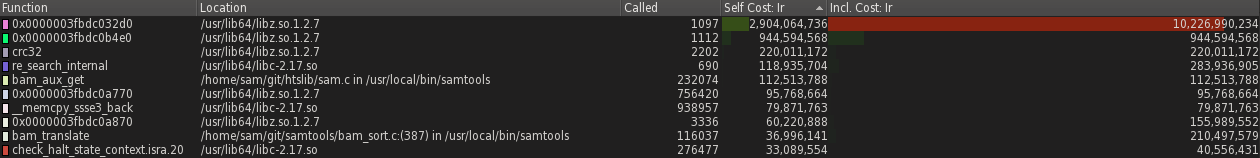
\includegraphics[width=1.0\textwidth]{callgrind_compressoutput_default}
    \caption[callgrind-default]{callgrind output following merge with default
    output compression}
    \label{fig:callgrind-default}
\end{figure}

\begin{figure}[htbp!]
    \centering
    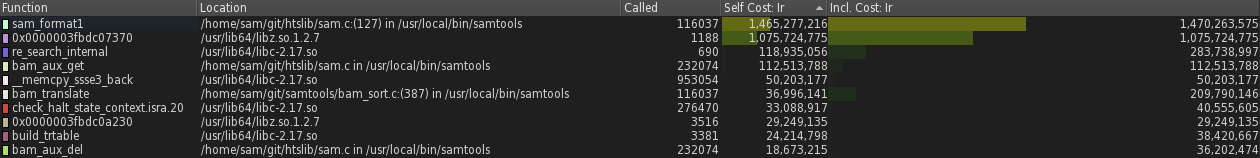
\includegraphics[width=1.0\textwidth]{callgrind_uncompressoutput}
    \caption[callgrind-uncompressed]{callgrind output following merge with
    uncompressed output}
    \label{fig:callgrind-uncompressed}
\end{figure}

% http://www.zlib.net/feldspar.html
Looking at a brief explanation of the deflate algorithm, it seems reasonable to
conclude the computational cost is rather asymmetric between compressing and
uncompressing - in that the effort is locating blocks to compress and in
comparison uncompressing is a reversible function on the known blocks.

Indeed, samtools merge specifies a -u option for uncompressed output and the
callgrind output (second image) indicates significantly less calls to zlib
functionality.

It remains to be seen whether this option will cut down the time needed for the
large merge job, perhaps this is merely a red herring and we’re yet to discover
the true speed trouble. In the meantime let’s see if sending this job to the
farm will work.


\subsubsection{The Red Herring}

% http://www.cs.utah.edu/dept/old/texinfo/as/gprof.html
... might be interesting to use gprof which is more
geared towards finding functions that spend all your execution time as opposed
to callgrind which I believe counts CPU instructions.

% http://paste.chippy.ch/woj.md
% https://github.com/samtools/htslib/blob/develop/sam.c#L1031
After re-compiling htslib and samtools with the -pg flag to enable such
profiling and executing the same previous merge command on the modest test set,
the output as parsed by gprof seems to indicate that the trouble lies with
bam\_aux\_get in htslib, with almost 50\% of the execution time being spent in
this particular function.

\begin{minted}[mathescape,
            %linenos,
            numbersep=5pt,
            %gobble=4,
            frame=lines,
            framesep=2mm]{c++}
    uint8_t *bam_aux_get(const bam1_t *b, const char tag[2])
    {
        uint8_t *s;
        int y = tag[0]<<8 | tag[1];
        s = bam_get_aux(b);
        while (s < b->data + b->l_data) {
            int x = (int)s[0]<<8 | s[1];
            s += 2;
            if (x == y) return s;
            s = skip_aux(s);
        }
        return 0;
    }
\end{minted}


% http://samtools.github.io/hts-specs/SAMv1.pdf
At a glance it seems that bam\_aux\_get receives a pointer to a BAM record and a
“tag”, an array of two characters representing an optional field as defined in
Section 1.5 of the SAM file spec.

The function then appears to fetch all these auxiliary tags and iterates over
each, comparing a transformation of that tag (x) to a pre-computed
transformation on the input tag (y).

% https://github.com/samtools/samtools/blob/2917ccdf34cd81b1327532b2db6e522fe871f054/bam_sort.c#L469
% https://github.com/samtools/samtools/blob/2917ccdf34cd81b1327532b2db6e522fe871f054/bam_sort.c#L484
% https://github.com/samtools/samtools/blob/2917ccdf34cd81b1327532b2db6e522fe871f054/bam_sort.c#L697
This would of course be inherently slow for files with many such tags;
especially given that the function is called twice for potentially each line in
a BAM file.


\subsubsection{The Plot Thickens}

% https://github.com/samtools/samtools/blob/2917ccdf34cd81b1327532b2db6e522fe871f054/bam_sort.c#L207
...as we increase the number of input files, the time taken to
read them in becomes non-linearly slower. Currently my money is on the seemingly
inefficient trans\_tbl\_init that appears to be called for each file, with the
current table of all previous files as an input...


\section{Calling}
\subsection{bcftools call}

Variant calling was briefly introduced as a concept in Part I
(See Section~\ref{sec:p1-concept:variants}). Calling for variants is the process
of finding differences between a reference sequence\footnote{Our analysis maps
    to the \textbf{hs37d5} reference sequence, used by the \textit{1000 Genomes
    Project Phase II}\citep{1k-refs}. \textbf{hs37d5} extends the \textbf{b37} genomic
    reference with "decoy sequences" that are designed to reduce false
    positives (incorrectly mapping to poorly referenced areas around centromeres for
    example\citep{biostar:decoy}), optimising it for variant
calling\citep{1k-slides}.} and a given sample\footnote{Technically to be confident
    you have an actual SNP as opposed to a variant (or incorrect read!), you'll
    need to see whether such variation occurs through a population of different
samples rather than just one.} or set of different samples.

The genotype likelihoods calculated by \textbf{samtools mpileup} in the previous
step of the pipeline represent a probability distribution of the bases seen
across all piledup samples at a particular location (site). This allows variant
calling algorithms to make an informed decision as to whether particular sites
actually contain a SNP or if a differing base is statistically unlikely to be a real
variant\footnote{Although it could also be a very low frequency variant...} with
the current data.

\textbf{bcftools call}\citep{man:bcftools-call}\citep{man:bcftools-call2} is the
successor to the 'consensus' variant caller included with the \textbf{samtools}
package and utilises \textbf{htslib} for improved file handling efficiency with
common genomic data formats.

%TODO all crohns samples...
%TODO writing is naff

Unfortunately during the initial testing of this step, using a pileup of all the
Goldilocks regions, the output contained only the standard header information
generated by \textbf{bcftools} and not a single record detailing a called
variant.  I discovered this was due to the \textbf{samtools mpileup} job being
completed without including a reference sequence, causing the \textit{REF}
(reference) column of the resulting \textbf{BCF} file to be populated with 'N':
an ambiguity code which translates to 'any
base'\citep{cornish1985nomenclature}\citep{liebecq1992biochemical}.

\textbf{bcftools call} does provide the \texttt{--M} flag for this scenario,
where the reference is described as a "masked reference". However attempting to
repeat calling with the flag set merely caused the command to produce a
segmentation fault instead of an empty output file. This appeared to be due to a
compatibility issue between the versions of \textbf{htslib} and
\textbf{bcftools} I was using on the \textbf{Farm}.

Finally this initial test of the calling component of our pipeline was able to
be completed in 66 minutes with an average memory usage of 11.97MB, resulting in
a 114MB compressed VCF file. In future runs, output size could be reduced by
generating a list of variants that appear in both the \textbf{GWAS} and
\textbf{iCHIP} Goldilocks regions (as these are the only variants we are
interested in anyway). This "targets" file actually uses the same format as the
\textbf{Variant Query Files} described in Section~\ref{sec:vqf} and should be
provided to \textbf{bcftools call}'s \texttt{--T} (\texttt{----targets-file})
option.


\section{Measuring Concordance}

...constructed another Python script...
...also could have used SNPConcordance Java lib...

...however as it was not possible to reach this stage, discussion on this is
considered outside the scope of this write-up...
